\chapter{Work Done}\label{C:workdone}

\section{Overview}

The ability to trace and perform several different analysis methods has been implemented. For this to be achieved, several factors had to be completed and explored in this chapter. The different types of analysis methods are explored in Section \ref{S:analysis}. How the tracing is performed is examined in Section \ref{S:trace}. While the creation of the framework is explored in Section \ref{S:framework}. Lastly, how the benchmarks were selected is looked at in Section \ref{S:bench}.

\section{Analysis Metrics}
\label{S:analysis}

The idea of a spectra was previously identified in Chapter \ref{C:intro}. A spectra is the method executions of a test which allows there to be several different types of spectra's. The main three spectra's examined are:

\begin{itemize}
\item Set of method executions - where every method execution is only taken into account once
\item List of method executions - where every method execution is taken into account
\item Calling Context - for each method call, the data contains a separate node for each call stack that the method was called with \cite{callingcontext}
\end{itemize}
These spectra's will be analysed through different metrics to determine the level of redundancy between two tests. In the next section, two different analysis metrics are introduced and examined.

The first metric is the Levenshtein distance between two tests spectra's. This metric is determining the minimal number of operations that can be done to make one tests spectra equal to another. These operations are inserting, deleting or substituting method calls and a cost is associated with completing an operation. The max difference is the size of the larger of the two spectra's. The amount of redundancy is calculated by dividing the cost of operations with the max difference in order to normalize the value.

If we look at an example where 'kitchen' is becoming compared to 'kitten' then we will have to do the following changes.

\begin{enumerate}
\item kitten $\rightarrow$ kitcen (Substitution of 't' with 'c')
\item kitcen $\rightarrow$ kitchen (Insertion of 'h' between 'c' and 'e')
\end{enumerate}

This shows the number of operations needed is 2, and the max is 7. Since it is a minimization metric, we can compute the redundancy as 1-2/7. So these two words contain 71\% redundant information. 

The second metric was determining the total difference between two spectra's. This metric disregarded the calling order of a spectra, which is comparable to looking at the coverage as done in several papers \cite{fraser2007redundancy} \cite{koochakzadeh2009test} \cite{zhang2011empirical} \cite{jeffrey2005test} as well a greedy longest common substructure algorithm. The metric sorts the method calls of a spectra in alphabetical order and increments a value by 1 for each difference there is between two tests spectra. Resulting in the total difference between two tests. This value is then divided by the max possible value, which would occur when every method call is different becoming the length of both spectra, to produce a normalized redundancy value.

Using the same example as above, we need to rearrange 'kitchen' and 'kitten' into alphabetical order before calculating the redundancy, 'cehiknt' and 'eikntt' respectively.

\begin{enumerate}
\item Remove 'c' from 'cehiknt', increment value by 1
\item 'e' is contained in both, remove from both
\item Remove 'h' from 'hiknt', increment value by 1
\item 'iknt' is contained in both, remove from both
\item Remove 't' from 't', increment value by 1
\end{enumerate}

The total difference between the two is 3. While the max would be if they were both completely different which is 13. This is also a minimization metric, therefore 1-3/13 will calculate the level of redundancy. The outcome being that the two words are 77\% redundant.



Maurer et al. \cite{koochakzadeh2009test} and Robinson et al. \cite{li2008static} found that test cases often had a set of methods that were in every test, such as setup and tear down. These common methods could create false positives. To understand why, a redundant test is one where it has the near or exact replication of another test. Since each method call within an spectra has the same weighting, the more setup and teardown calls made means that the execution stage has decreased weighting overall. So the idea in weighting is to increase the 'importance' of lower frequency method calls by discarding the top 20\% method calls. Allowing weighting to be added into a spectra, where the spectra will ignore these method calls.

\section{Tracing}
\label{S:trace}

David Pearce's language Whiley is written in Java. Therefore it was decided to use Java to trace a tests spectra. There are two viable options, Java Debugging Interface (JDI) or AspectJ. JDI is similar to using a observer pattern. When a method is called, the listening trace class will be notified. On the other hand, AspectJ utilises byte code weaving; where an aspect is adding behaviour to existing code without modifying the code itself. It uses a point cut to identify what code is weaved and where in the code \cite{aspectwiki}. AspectJ allows for several methods to achieve tracing through byte code weaving:

\begin{itemize}
\item Compile time:
The classes are compiled with the aspect weaved into them. So that when the jar is executed, the methods have the byte code from the aspect weaved into it already \cite{weaving}.
\item Load time:
This involves binary weaving deferred until the point in which a class loader will attempt to load in a class file and define it to the java virtual machine (JVM) \cite{weaving}.
\end{itemize}

Load time allowed for ease of use when working with external benchmarks as it only required AspectJ's class loader to be used instead of rebuilding the benchmarks with the AspectJ compiler.

In regard to JDI or AspectJ. AspectJ allows for stronger ability to choose which methods to record and gives more ability to retrieve the parameters however JDI was faster to execute. The decision to use AspectJ was based off a trade off between more information and performance. The analysis framework was able to be altered to increase the performance of it, so having the extra information that AspectJ gave was more important than an taking less time to execute.

\section{Framework}
\label{S:framework}

Every spectra has to be compared to every other spectra in order to identify redundant test cases. The metrics identified become computationally heavy with thousands of test cases containing a spectra consisting of tens of thousands of methods calls. To perform an analysis on that scale would take a substantial amount of time. A pipeline combined with reduction centered strategies was determined to be the best solution.

A pipeline approach is shown in figure \ref{fig:pipeline}. Where each method in the pipeline will be an analysing stage. The analysing stages can be set by the user within a properties file, where they can select the spectra type, analysis metric to use and level of redundancy for each.

\begin{figure}[h]
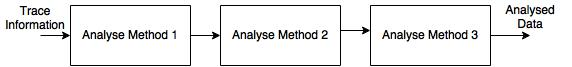
\includegraphics[width=\textwidth]{Pipeline.jpg}
\caption{Pipeline}
\label{fig:pipeline}
\end{figure}

There were two approaches that were used to reduce the amount of analysis time. They were - implementing a 'bloom filter' and using concurrent execution. 

A bloom filter is a test where it determines whether an element is a member of a set or not, returning either "possibly in set" or "definitely not in set" \cite{bloomfilterwiki}. In this case, it was used to determine whether the set of method calls for two tests were similar or not. The similarity and analysis type are set within a properties file. Looking at the set of method calls, rather than a list meant the number of comparisons decreased. Using a 99 percent similarity for the 'bloom filter' on the wyc package of Whiley, this meant the next analysis stage had 232 comparisons, rather than 187922. This approach was used under the hypothesis that the following is true.

$A, B, C, D \neq A, D, E, F, G$

$A, B, C, D \approx A, B, C, D, E$

In the first case the two tests would be not be redundant test’s due to having a high difference in method calls. However, there is a chance that the second test may be redundant so it implies more computational heavy analysis should be done on it, such as using a list spectra. 

Concurrent execution was implemented by splitting the test cases up into 8 different parts, each part knew the test cases that it had to compare. A new thread was run to execute the comparisons, making the implementation relatively easy. The concurrent execution lead to a decrease in roughly 2 times the time taken to analyse the spectra's. 
The analysis time had been reduced drastically, however, to run a pipeline the test suite had to be re run each time. With up to tens of thousands of tests, this could take several hours. The solution, save the spectra data to disk. Allowing for the spectra information to be reloaded and analysed without the tests being re run.

\section{Benchmarks}
\label{S:bench}
Suitable benchmarks had to be found to test the different metrics on; this was harder than it seemed. The benchmarks had to meet a criteria where they were Java based, had large number of test cases (100 +) and were open source. Although there were over 10 potential benchmarks, the ability to use them depended on their build process. If they used Maven, it was difficult to create a jar that contained the tests and often meant that the amount of effort needed to get a working benchmark was higher than the benefit from it. This eliminated several potential benchmarks and left the Ant and gradle built projects. 

The current set of benchmarks is as follows:

\begin{itemize}
\item Whiley
\item Java Compiler Kit
\item Jasm
\item Spring - Core
\item Metric-x - Core
\item Ant
\end{itemize}